  %%%%%%%%%%%%%%%%%%%%%%%%%%%%%%%%%%%%%%%%%%%%%%%%%%%%%%%%%%%%%%%%%%%%%%
% LaTeX Example: Project Report

%%% Preamble
\documentclass[paper=a4, fontsize=11pt, abstract=on]{scrartcl}
\usepackage[T1]{fontenc}
\usepackage{fourier}
\usepackage{tabularx}
\usepackage[utf8]{inputenc}
\usepackage{hyperref}





\usepackage{listings}
\usepackage{color}

\definecolor{dkgreen}{rgb}{0,0.6,0}
\definecolor{gray}{rgb}{0.5,0.5,0.5}
\definecolor{mauve}{rgb}{0.58,0,0.82}
\lstset{frame=tb,
  language=[Visual]C++,
  aboveskip=3mm,
  belowskip=3mm,
  showstringspaces=false,
  columns=flexible,
  basicstyle={\small\ttfamily},
  numbers=none,
  numberstyle=\tiny\color{gray},
  keywordstyle=\color{blue},
  commentstyle=\color{dkgreen},
  stringstyle=\color{mauve},
  breaklines=true,
  breakatwhitespace=true,
  tabsize=3
}
\usepackage{graphicx}
\usepackage{caption}
\usepackage{subcaption}

\usepackage[english]{babel}															% English language/hyphenation
\usepackage[protrusion=true,expansion=true]{microtype}	
\usepackage{amsmath,amsfonts,amsthm} % Math packages

\usepackage{url}
%\usepackage[hang, small,labelfont=bf,up,textfont=it,up]{caption}


%%% Custom sectioning
\usepackage{sectsty}
\allsectionsfont{\normalfont\scshape}
\usepackage{float}
\usepackage{amsmath}
\usepackage{mathtools}
\usepackage{ragged2e}

\usepackage{nomencl}
\makenomenclature

%%% Custom headers/footers (fancyhdr package)
\usepackage{fancyhdr}
\pagestyle{fancyplain}
\fancyhead{}											% No page header
\fancyfoot[L]{}											% Empty 
\fancyfoot[C]{}											% Empty
\fancyfoot[R]{\thepage}									% Pagenumbering
\renewcommand{\headrulewidth}{0pt}			% Remove header underlines
\renewcommand{\footrulewidth}{0pt}				% Remove footer underlines
\setlength{\headheight}{13.6pt}
   \renewcommand*\abstractname{Summary}

%%% Equation and float numbering
\numberwithin{equation}{section}		% Equationnumbering: section.eq#
\numberwithin{figure}{section}			% Figurenumbering: section.fig#
\numberwithin{table}{section}				% Tablenumbering: section.tab#


%%% Maketitle metadata

\newcommand{\horrule}[1]{\rule{\linewidth}{#1}} 	% Horizontal rule

\title{
		%\vspace{-1in} 	
		\usefont{OT1}{bch}{b}{n}
		\normalfont \normalsize \textsc{} \\ [25pt]
		
\includegraphics[width=0.3\linewidth]{ubc.png} \\
		%
\includegraphics[width=0.4\linewidth]{tru}		
		\horrule{0.5pt} \\[0.2cm]
		\huge Programming Assignment \#3 : Solving Incompressible Energy Equation  \\
		\horrule{2pt} \\[0.005cm]
}
\author{
		\normalfont 								\normalsize
        Jerin Roberts\\[-5pt]		\normalsize
        \today
}
\date{}




%%% Begin document
\begin{document}
\maketitle
\begin{center}
\begin{tabular}{l r}


Supervisor: & Dr. Carl Ollivier-Gooch  \\ % supervisor
Locations: & University of British Columbia


\end{tabular}
\end{center}



\newpage
\tableofcontents
\listoffigures
\listoftables
\newpage
\lstset{language=[Visual]C++}
\section{Introduction}



 The are many physical phenomenons in physics and engineering that require linear and non-linear partial differential equations to described the true nature of the system. Solving these systems analytically and finding exact solutions for these equations can be difficult and often require simplifications that ultimately don't fully represent the problem being investigated. Numerical methods for solving PDE's provides a means for finding approximations to the exact solutions without having to make sacrificial simplifications. With recent advancements in computational technology numerical methods can now be easily applied to large and difficult problems that would otherwise be impossible to solve. 
\subsection{Problem Overview}
Numerical problems are essentially solved by breaking the entire solution domain into small discrete points (mesh) and finding the solution at or around these areas. Each point requires the solving the differential equations that represent physical phenomenon being investigated. Since the exact solution cannot be computed, it is instead approximated using various techniques and methods. In this assignment the 2D incompressible laminar energy equation is applied to a rectangular channel for a given velocity field. The problem will employ an second ordered centered flux calculation with both implicit and explicit euler timer advance methods. The implicit method will be solved using approximate factorization and Gauss-Jordan elimination via the Thomas algorithm. Boundary conditions will be implement using ghost cells allowing the interior scheme to remain the same during calculation of bordering cells. The ghost cells are calculated such the boundary condition is enforced at $i=1/2$.



\section{Implementation}
\subsection{Program Overview}
The C/C++language was selected for this programming assignment. The scripts were compiled using g++/gcc version 5.4.0 on Ubuntu 16.04.02 and are available in the attached zip or for clone via the link provided: \url{https://github.com/j16out/cfd510} . The program itself is broken into 3 pieces and two levels to produce a modular set that makes it easier to apply to different problems. The highest level contains the "macro" or the main function which can be modified for different problems. 

\begin{table}[H]
\begin{center}
    \begin{tabular}{ | p{0.23\linewidth} | p{0.6\linewidth} |}
 \hline  
     \RaggedRight \textbf{Function}
    &\RaggedRight \textbf{Purpose}
    \\ \hline  
           \RaggedRight set\_ array\_ size() 
    &\RaggedRight Set size of array if not default(160x160)
    \\ \hline 
           \RaggedRight set\_ ghostcells()
    &\RaggedRight Set Ghost cells and update boundary conditions
    \\ \hline 
    \RaggedRight set\_ zero()
    &\RaggedRight Zero entire array including ghost cells
    \\ \hline 
           \RaggedRight set\_ intial\_ cond()
    &\RaggedRight Set initial condition
    \\ \hline 
           \RaggedRight print\_ array()
    &\RaggedRight Prints array in terminal style output
    \\ \hline 
           \RaggedRight get\_ FIarray()
    &\RaggedRight Evaluates Flux for array interior cells
    \\ \hline 
           \RaggedRight get\_ RK2()
    &\RaggedRight performs RK2 iteration 1 or 2 stage
    \\ \hline 
      \RaggedRight get\_ FIarray\_ 1stcell()
    &\RaggedRight Calculates flux at 1st interior cell
    \\ \hline 
    \RaggedRight  get\_ surcells()
    &\RaggedRight Gets current solution of neighboring cells
    \\ \hline 
    \RaggedRight  mv\_ SOL2\_ to\_ SOL1()
    &\RaggedRight moves updated solution to first stage array
    \\ \hline 
    \RaggedRight  solve\_ arrayRK2()
    &\RaggedRight Performs are steps to solve problem
    \\ \hline 
    \RaggedRight get\_ l1norm()
    &\RaggedRight Returns $L^1$ norm error
      \\ \hline 
    \RaggedRight get\_ l2norm()
    &\RaggedRight Returns $L^2$ norm error between two arrays of equal size
    \\ \hline 
    \RaggedRight get\_ linf\_ norm() 
    &\RaggedRight Returns $L^{\infty}$ norm error between two arrays of equal size
    \\ \hline 
    \RaggedRight set\_ analytic() 
    &\RaggedRight Set array values to predefined exact solution
    \\ \hline 
   
   
    
    \end{tabular}
\end{center} 
\caption{List of Program Functions}
\label{func} 
\end{table}

The numerical directory contains numerical.cpp script and its header file numerical.hpp. This set contains all the functions necessary for solving the problem numerically. Table \ref{func} displays all functions with a short description of each. The vroot directory contains the scripts necessary for drawing data. These scripts make use of the ROOT-v6 libraries. ROOT is a popular data analysis framework primarily written in C++ and Phython. For more information on ROOT libraries visit the link provided: \url{https://root.cern.ch/} .
The functions act on a structure called $carray$ which contains the solution domain array and its various parameters. The struct contains the main array, its defined working area (mesh size), data storage vectors, iteration count, and the represented dimension between points. Having these organized in a struct provides a compact way of passing and modifying the array and all its pertinent parameters. The outline of the struct used for the energy equation problem is shown below.

 

\begin{lstlisting}
struct carray{
//arrays
double f1 [maxx][maxy];//flux or temp space
double T1 [maxx][maxy];//Temperature
double v1 [maxx][maxy];//x velocity
double u1 [maxx][maxy];//y velocity
//array attributes
int sizex = maxx;
int sizey = maxy;
double DIMx = 0.0;
double DIMy = 0.0;
//time
double ctime = 0;
};
\end{lstlisting}
 
\subsection{Flux Calculation}


 The program was built and tested in small components to ensure its correctness. The flux integral without the source term was run and compared to the exact solution for the flux integral as displayed in equation \ref{eflux}. This exact integral can be approximated by a scheme of cell volume averages as shown in equation \ref{xflux} for x and \ref{yflux}. The problem will employ a second ordered centered flux calculation which is found on the RHS of the discretized energy equation.


\begin{equation}
\label{eflux}
\iint \Bigg(u\frac{\partial T}{\partial xt} + v\frac{\partial T}{\partial y}-\frac{\bigtriangledown^2T}{Re Pr}\Bigg)dA
\end{equation}



  \begin{equation}
\label{xflux}
\frac{-1}{\triangle x}\Bigg(\frac{u_{i+1,j}\overline{T}_{i+1,j}^n-u_{i-1,j}\overline{T}_{i-1,j}^n}{2}-\frac{1}{Re Pr}\Bigg(\frac{\overline{T}_{i+1,j}^n-2\overline{T}_{i,j}^n+\overline{T}_{i-1,j}^n}{2\triangle x}\Bigg)\Bigg)
\end{equation}

 \begin{equation}
\label{yflux}
 \frac{1}{\triangle y}\Bigg(\frac{v_{i,j+1}\overline{T}_{i,j+1}^n-u_{i,j-1}\overline{T}_{i,j-1}^n}{2}-\frac{1}{Re Pr}\Bigg(\frac{\overline{T}_{i,j+1}^n-2\overline{T}_{i,j}^n+\overline{T}_{i,j-1}^n}{2\triangle y}\Bigg)\Bigg)
\end{equation}

The flux was calculated using the function $compute\_ flux()$, which is shown below. The function calls two other functions which grab the necessary data using the $surr$ struct from the current solution. The flux calculated using $calc\_ newcell()$ is then stored on the $carray$ struct under the $f1$ array.

\begin{lstlisting}
void compute_Flux(carray & myarray)
{
surr mysurr;
for(int j = 1; j < myarray.sizey-1; ++j)
{
    for(int i = 1; i < myarray.sizex-1; ++i)
    {
    //----get surrounding cells and compute new cell----//
    get_nsurcells(myarray, i, j, mysurr);
    //-----update current cell----//
    double newcell = calc_newcell(myarray, mysurr);    
    myarray.f1[i][j] = newcell;   
    }
}
}
\end{lstlisting}



\begin{table}[H]
\begin{center}
    \begin{tabular}{ | p{0.13\linewidth} | p{0.2\linewidth} |p{0.1\linewidth} |p{0.1\linewidth} |p{0.1\linewidth} |}
 \hline  
     \RaggedRight \textbf{Mesh Size}
    &\RaggedRight \textbf{$L^2$norm}
    &\RaggedRight \textbf{$\triangle x$}
    &\RaggedRight \textbf{Order}
    \\ \hline  
           \RaggedRight 10 x 10
    &\RaggedRight 8.773$*10^{-1}$
    &\RaggedRight 0.1
    &\RaggedRight -
    \\ \hline 
    \RaggedRight 20 x 20
    &\RaggedRight 2.230 $*10^{-1}$
    &\RaggedRight 0.05
    &\RaggedRight 1.981
    \\ \hline 
           \RaggedRight 40 x 40
    &\RaggedRight 9.942 $*10^{-2}$
    &\RaggedRight 0.025
    &\RaggedRight 1.986
    \\ \hline 
           \RaggedRight 80 x 80
    &\RaggedRight 1.401$*10^{-2}$
    &\RaggedRight 0.0125
    &\RaggedRight 1.991
    \\ \hline       
   \end{tabular}
\end{center} 
\caption{Table of $L^2$ norms for increasing mesh size of flux integral}
\label{norm1} 
\end{table}

The correctness of the flux integral was validated using the exact computer flux. The $L_2$ norms for the flux calculation are displayed in table \ref{norm1}. The order of accuracy for the scheme was determined using the log log method as displayed in figure \ref{order}. The order of accuracy for this scheme was estimated to be 2nd order accurate based on the $L_2$ data from 8 different meshes.     
    
  

\begin{figure}[H]
\centering
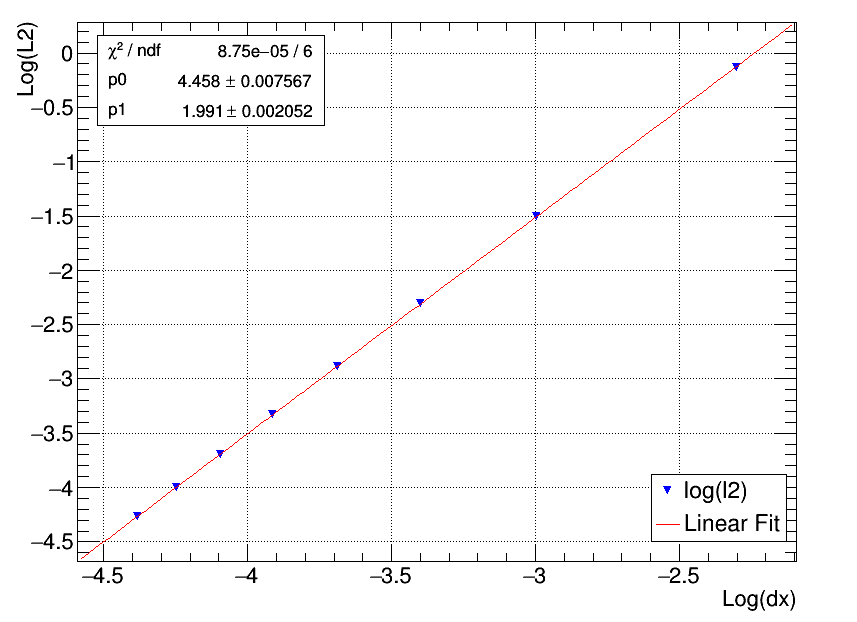
\includegraphics[width=0.85\linewidth]{order}
\caption{Calculated Order of Accuracy without source}
\label{ord}
\end{figure}


This matches what was expect by implementing a 2nd order interior flux evaluation and boundary schemes. It should be noted as seen in figure \ref{qq22} the relative error decreases when refining the mesh. This is expect as the numerical solution is a discrete representation of the continuous exact solution. 

 




\subsection{Source Term Validation}

\begin{figure}[H]
\centering
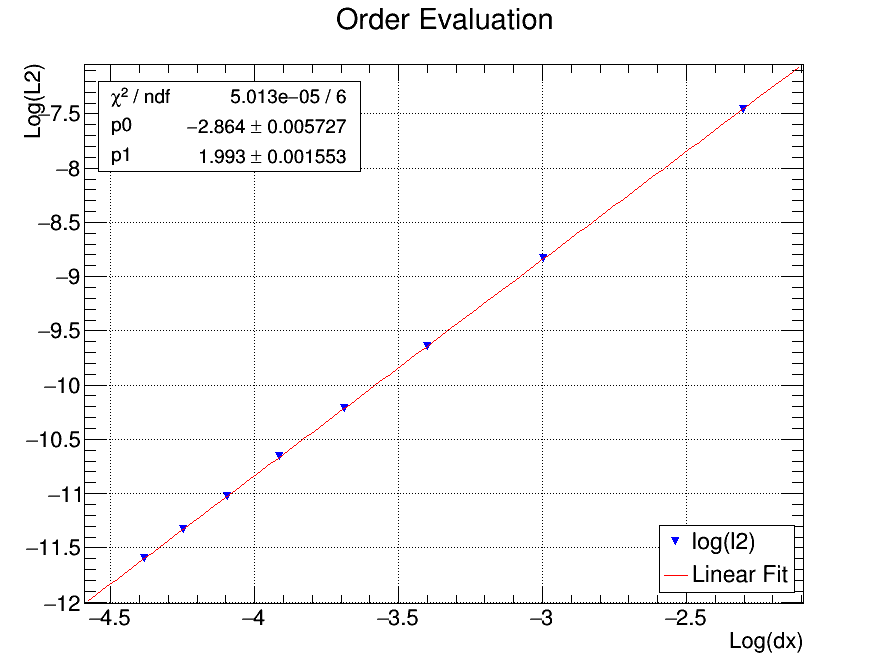
\includegraphics[width=0.85\linewidth]{source}
\caption{Calculated Order of Accuracy of only source term}
\label{ord}
\end{figure}




\begin{figure}[H]
\centering
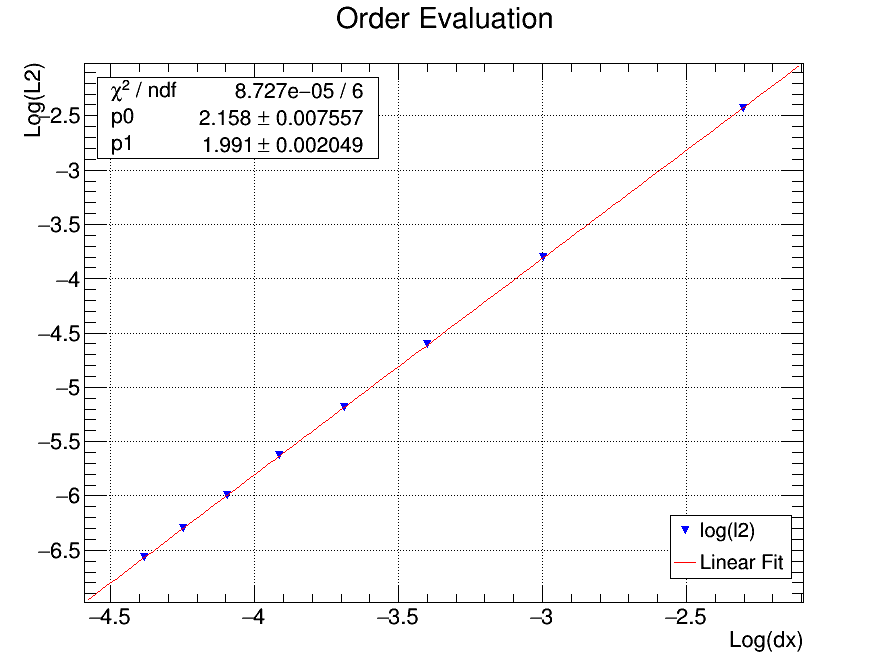
\includegraphics[width=0.85\linewidth]{orderws}
\caption{Calculated Order of Accuracy with of flux integral with source}
\label{ord}
\end{figure}



 \begin{table}[H]
\begin{center}
    \begin{tabular}{ | p{0.13\linewidth} | p{0.2\linewidth} |p{0.1\linewidth} |p{0.1\linewidth} |p{0.1\linewidth} |}
 \hline  
     \RaggedRight \textbf{Mesh Size}
    &\RaggedRight \textbf{$L^2$norm}
    &\RaggedRight \textbf{$\triangle x$}
    &\RaggedRight \textbf{Order}
    \\ \hline  
           \RaggedRight 10 x 10
    &\RaggedRight 8.796$*10^{-2}$
    &\RaggedRight 0.1
    &\RaggedRight -
    \\ \hline 
    \RaggedRight 20 x 20
    &\RaggedRight 2.235 $*10^{-2}$
    &\RaggedRight 0.05
    &\RaggedRight 1.981
    \\ \hline 
           \RaggedRight 40 x 40
    &\RaggedRight 5.613 $*10^{-3}$
    &\RaggedRight 0.025
    &\RaggedRight 1.985
    \\ \hline 
           \RaggedRight 80 x 80
    &\RaggedRight 1.405$*10^{-3}$
    &\RaggedRight 0.0125
    &\RaggedRight 1.991
    \\ \hline 
      
 
    
    
    \end{tabular}
\end{center} 
\caption{Table of $L^2$ norms for increasing mesh size of flux integral with source}
\label{norm} 
\end{table}


\subsection{Explicit Time scheme}
\begin{figure}[H]
\centering
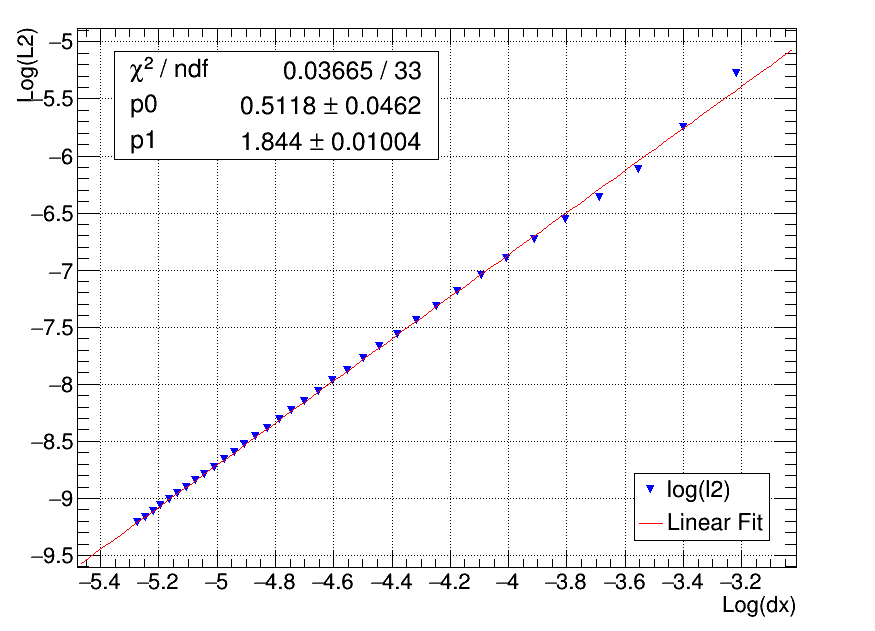
\includegraphics[width=0.85\linewidth]{orderexplicit}
\caption{Calculated Order of Accuracy using explicit method for varying mesh sizes}
\label{ord}
\end{figure}


 \begin{table}[H]
\begin{center}
    \begin{tabular}{ | p{0.13\linewidth} | p{0.2\linewidth} |p{0.1\linewidth} |p{0.1\linewidth} |p{0.1\linewidth} |}
 \hline  
     \RaggedRight \textbf{Mesh Size}
    &\RaggedRight \textbf{$L^2$norm}
    &\RaggedRight \textbf{$\triangle x$}
    &\RaggedRight \textbf{Order}
    \\ \hline  
           \RaggedRight 25 x 10
    &\RaggedRight 5.11$*10^{-3}$
    &\RaggedRight 0.2
    &\RaggedRight -
    \\ \hline 
    		\RaggedRight 50 x 20
    &\RaggedRight 1.19 $*10^{-3}$
    &\RaggedRight 0.1
    &\RaggedRight 1.855
    \\ \hline 
           \RaggedRight 100 x 40
    &\RaggedRight  3.46  $*10^{-4}$
    &\RaggedRight 0.05
    &\RaggedRight 1.845
    \\ \hline 
           \RaggedRight 200 x 80
    &\RaggedRight 9.97$*10^{-5}$
    &\RaggedRight 0.025
    &\RaggedRight 1.844
    \\ \hline 
      
 
    
    
    \end{tabular}
\end{center} 
\caption{Table of $L^2$ norms for increasing mesh size of explicit method}
\label{norm} 
\end{table}


\subsection{implicit method}



\begin{figure}[H]
\centering
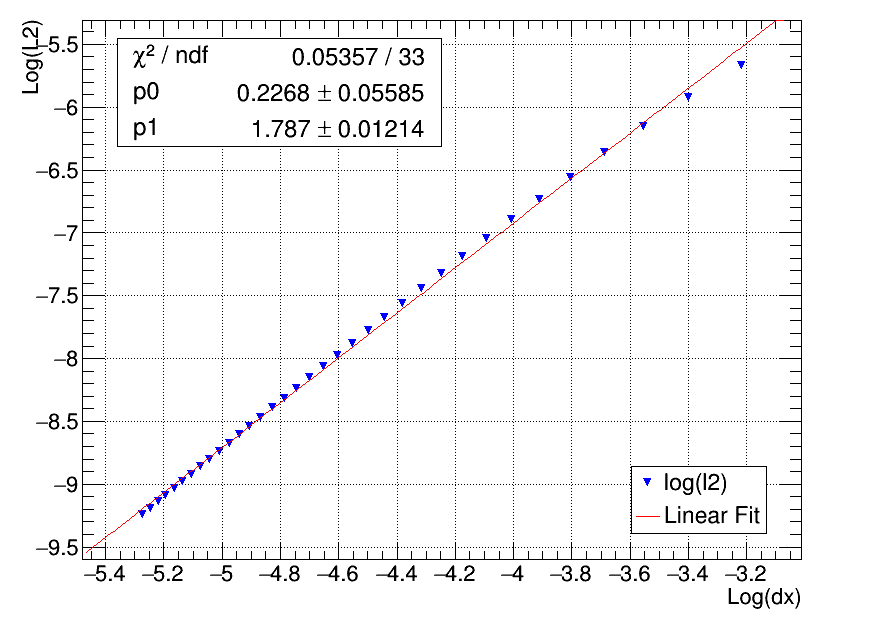
\includegraphics[width=0.85\linewidth]{orderimp}
\caption{Calculated Order of Accuracy using implicit method for varying mesh sizes}
\label{ord}
\end{figure}






 \begin{table}[H]
\begin{center}
    \begin{tabular}{ | p{0.13\linewidth} | p{0.2\linewidth} |p{0.1\linewidth} |p{0.1\linewidth} |p{0.1\linewidth} |}
 \hline  
     \RaggedRight \textbf{Mesh Size}
    &\RaggedRight \textbf{$L^2$norm}
    &\RaggedRight \textbf{$\triangle x$}
    &\RaggedRight \textbf{Order}
    \\ \hline  
           \RaggedRight 25 x 10
    &\RaggedRight 3.48$*10^{-3}$
    &\RaggedRight 0.2
    &\RaggedRight -
    \\ \hline 
    		\RaggedRight 50 x 20
    &\RaggedRight 1.19 $*10^{-3}$
    &\RaggedRight 0.1
    &\RaggedRight 1.761
    \\ \hline 
           \RaggedRight 100 x 40
    &\RaggedRight  3.44  $*10^{-4}$
    &\RaggedRight 0.05
    &\RaggedRight 1.775
    \\ \hline 
           \RaggedRight 200 x 80
    &\RaggedRight 9.97$*10^{-5}$
    &\RaggedRight 0.025
    &\RaggedRight 1.787
    \\ \hline 
      
 
    
    
    \end{tabular}
\end{center} 
\caption{Table of $L^2$ norms for increasing mesh size of implicit method}
\label{norm} 
\end{table}
\subsection{Efficiency}



\subsection{Final Problem}

\begin{table}[H]
\begin{center}
    \begin{tabular}{ | p{0.2\linewidth} | p{0.2\linewidth} |}
 \hline  
     \RaggedRight \textbf{Values}
    &\RaggedRight \textbf{${dT}/{dy}$}
     \\ \hline 
      \RaggedRight $N_1, N_2, N_3$ 
    &\RaggedRight 200, 100, 50
    \\ \hline  
           \RaggedRight $r_{21}$ 
    &\RaggedRight 2.0
    \\ \hline 
           \RaggedRight $r_{32}$
    &\RaggedRight 2.0 
    \\ \hline 
           \RaggedRight ${dT_1}/{dy}$
    &\RaggedRight 1.123628 
    \\ \hline 
           \RaggedRight ${dT_2}/{dy}$
    &\RaggedRight 1.118769 
    \\ \hline
       \RaggedRight ${dT_3}/{dy}$
    &\RaggedRight 1.110733
    \\ \hline 
           \RaggedRight $p$
    &\RaggedRight 0.725830 
    \\ \hline 
       \RaggedRight $P_{ext}^{21}$
    &\RaggedRight 1.131059 
    \\ \hline  
    \RaggedRight $e_a^{21}$
    &\RaggedRight $\%$0.4324
    \\ \hline 
       \RaggedRight $e_{ext}^{21}$
    &\RaggedRight $\%$0.6570  
    \\ \hline 
       \RaggedRight $GCI_{fine}^{21}$
    &\RaggedRight $\%$0.8267
    \\ \hline 

    
    
    \end{tabular}

\end{center} 
\caption{Table of $L^2$ norms for increasing mesh size}
\label{norm1} 
\end{table}


max slope: 1.123628 at 12.450000
max slope: 1.118769 at 12.500000
max slope: 1.110733 at 12.200000


\begin{table}[H]
\begin{center}
    \begin{tabular}{ | p{0.13\linewidth} | p{0.2\linewidth} |p{0.2\linewidth}|}
 \hline  
     \RaggedRight \textbf{Mesh Size}
    &\RaggedRight \textbf{${dT}/{dy}$}
    &\RaggedRight \textbf{Channel x}
    \\ \hline  
           \RaggedRight 50 x 20
    &\RaggedRight 1.110733
      &\RaggedRight 12.20
    \\ \hline 
    		\RaggedRight 100 x 40
    &\RaggedRight 1.118769
    &\RaggedRight 12.5
    \\ \hline 
           \RaggedRight 200 x 80
    &\RaggedRight  1.123628
    &\RaggedRight 12.45
    \\ \hline 
   
    \end{tabular}
\end{center} 
\caption{Table of $L^2$ norms for increasing mesh size of implicit method}
\label{norm} 
\end{table}

\begin{figure}[H]
\centering
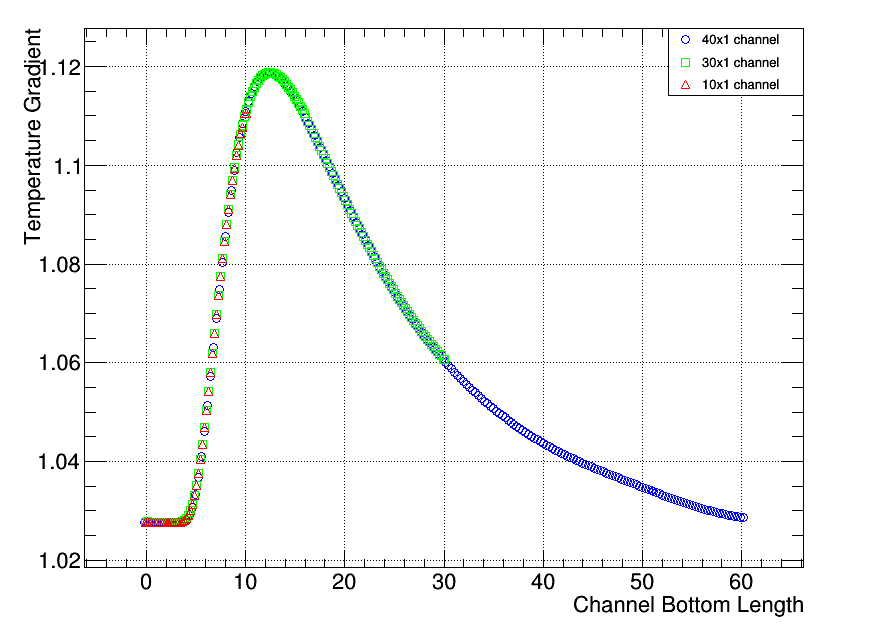
\includegraphics[width=0.85\linewidth]{chan}
\caption{Displays temperature gradient at bottom wall as a function of the channel length for varying channel lengths}
\label{ord}
\end{figure}

\begin{figure}[H]
\centering
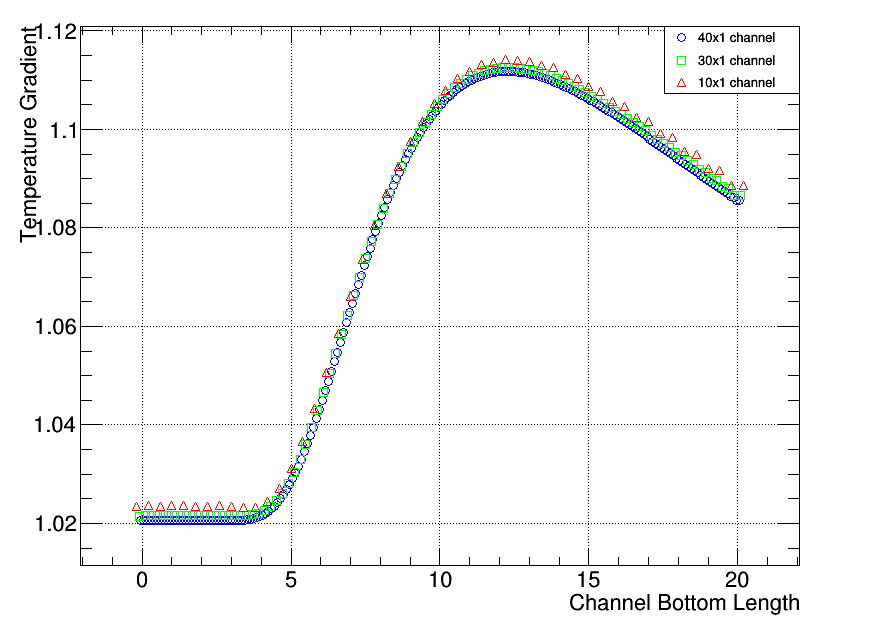
\includegraphics[width=0.85\linewidth]{chan2}
\caption{Displays the effect of mesh refinement on gradient solution}
\label{ord}
\end{figure}

\section{Conclusion}
This project provides great insight into the internal algorithms used for calculating numerical solutions for time varying problems. The Wave Equation problem provided a great platform for developing and testing the program. Having the analytic solution really help fine tune the program and helped given an idea on how accurate the solutions could be. Investigating the error and how it changes relative to boundaries and mesh sizes will provides insight on how the methods should be applied to bigger problems to minimize time and error. Stability analysis provided a great means for understanding the computational limits of the program in terms of speed. Numerical methods provide a great way of solving difficult problems and until new methods are discovered for finding exact solution will remain the main method for finding solutions to difficult problems. 






\appendix
\section{Appendix} \label{App:Appendix}
\subsection{wave.cpp}
\begin{lstlisting}
/*-------------------------------------------------------------------------------//
Main Program for finding solutions for wave equation. Employs a RK2 time advance 
with 2nd order upwind flux scheme.


Jerin Roberts 2016
compiled using g++/gcc version 5.4.0 on Ubuntu 16.04.02 and are available for clone 
via the link provided: url{https://github.com/j16out/
//-------------------------------------------------------------------------------*/


#include <vector>
#include <iostream>
#include <cstdlib>
#include <fstream>
#include <string>
#include <vector>
#include <algorithm>
#include <sstream>
#include <math.h> 
#include "TApplication.h"
#include "vroot/root.hpp"
#include "numerical/numerical.hpp"

using namespace std;




int main(int argc, char **argv)
{


carray wave1;//my main array
carray analytic1;
carray wave2;//my main array
carray analytic2;
carray wave3;//my main array
carray analytic3;
carray wave4;//my main array
carray analytic4;
carray wave5;//my main array
carray analytic5;
carray wave6;//my main array
carray analytic6;


//set size


//set array size or default used 162x162
set_array_size(wave1, 20, 1, 1.0, 0);//array, xsize, ysize, dimension
set_array_size(wave2, 40, 1, 1.0, 0);
set_array_size(wave3, 80, 1, 1.0, 0);
set_array_size(wave4, 160, 1, 1.0, 0);//array, xsize, ysize, dimension
set_array_size(wave5, 320, 1, 1.0, 0);
set_array_size(wave6, 686, 1, 1.0, 0);

set_array_size(analytic1, 20, 1, 1.0, 0);
set_array_size(analytic2, 40, 1, 1.0, 0);
set_array_size(analytic3, 80, 1, 1.0, 0);
set_array_size(analytic4, 160, 1, 1.0, 0);
set_array_size(analytic5, 320, 1, 1.0, 0);
set_array_size(analytic6, 686, 1, 1.0, 0);




//print_array(analytic);



//set intial conditions


set_zero(wave1);
set_intial_cond(wave1);
//print_array(wave1);//print array in terminal
set_zero(wave2);
set_intial_cond(wave2);

set_zero(wave3);
set_intial_cond(wave3);

set_zero(wave4);
set_intial_cond(wave4);
//print_array(wave1);//print array in terminal
set_zero(wave5);
set_intial_cond(wave5);

set_zero(wave6);
set_intial_cond(wave6);



float l2 = 0;

//---------------------solve array1----------------------//
solve_arrayRK2(wave1, 1.0, 0.4);//array,time,cfl
set_analytic(analytic1, wave1);
l2 = get_l2norm(wave1, analytic1);
wave1.l2norm.push_back(l2);
//cout << "Solution: " << get_solution(poisson1) << "\n";



//---------------------solve array2----------------------//
solve_arrayRK2(wave2, 1.0, 0.4);
set_analytic(analytic2, wave2);
l2 = get_l2norm(wave2, analytic2);
wave1.l2norm.push_back(l2);


//---------------------solve array2----------------------//
solve_arrayRK2(wave3, 1.0, 0.4);
set_analytic(analytic3, wave3);
l2 = get_l2norm(wave3, analytic3);
wave1.l2norm.push_back(l2);

//---------------------solve array1----------------------//
solve_arrayRK2(wave4, 1.0, 0.4);//array,time,cfl
set_analytic(analytic4, wave4);
l2 = get_l2norm(wave4, analytic4);
wave1.l2norm.push_back(l2);
//cout << "Solution: " << get_solution(poisson1) << "\n";



//---------------------solve array2----------------------//
solve_arrayRK2(wave5, 1.0, 0.4);
set_analytic(analytic5, wave5);
l2 = get_l2norm(wave5, analytic5);
wave1.l2norm.push_back(l2);


//---------------------solve array2----------------------//
solve_arrayRK2(wave6, 1.0, 0.4);
set_analytic(analytic6, wave6);
l2 = get_l2norm(wave6, analytic6);
wave1.l2norm.push_back(l2);



//----------------------Draw Data---------------------//

if(1)//start root application
{
	TApplication theApp("App", &argc, argv);//no more than two subs 
	draw_graph_q1(wave1, wave2, wave3, analytic1, analytic2, analytic3);   
	theApp.Run();
}

 //draw_graph_wave1(wave1, wave2, wave3);


//end
}

\end{lstlisting}
\subsection{numerical.hpp}
\begin{lstlisting}
#ifndef numerical_INCLUDED
#define numerical_INCLUDED


#include <vector>
#include <iostream>
#include <cstdlib>
#include <fstream>
#include <string>
#include <vector>
#include <algorithm>
#include <sstream>
#include <math.h> 
#include <iomanip>

using namespace std;

#define BIG 10000
#define maxx 8000
#define maxy 3
#define PI 3.141592654



struct carray{
//arrays
float mcellSOL [maxx][maxy];//first stage and solution mesh
float mcellSOL2 [maxx][maxy];//second stage solution mesh
float mcellFI [maxx][maxy];//first stage flux
float mcellFI2 [maxx][maxy];//second stage flux

//array attributes
int sizex = maxx;
int sizey = maxy;
float DIM1 = 0;

//current time 
float tstep = 0;
float ctime = 0;

//data storage specific to array
vector<float> l2norm;
vector<float> l1norm;
vector<float> linfnorm;
vector<float> diff;

//temporary cells to store
float Tim2_j=0.0;
float Tim1_j=0.0;
float Ti_j=0.0;
float Tip1_j=0.0;

//scheme
int scheme = 0;

};

//--------------------Init Arrays-----------------------------------------//

void set_array_size(carray & myarray, int x, int y, float DIM, int scheme);//set array size

void set_zero(carray & myarray);//zero entire array

void print_array(carray & myarray);//print array in terminal



//-------------------Boundary and Intial Conditions------------------------//

void set_ghostcells(carray & myarray);//set ghost cells

void set_intial_cond(carray & myarray);

void set_intial_cond2(carray & myarray);

//--------------------RK2 solver functions----------------------------------//

void get_FIarray(carray & myarray, int stage);//get all FI for array for specific stage

void get_FIarray_1stcell(carray & myarray, int stage);

void get_surcells(carray & myarray, int i, int j, int stage);//obtain values of surrounding cells stage defines were result stored

void get_RK2(carray & myarray, int stage);

void mv_SOL2_to_SOL1(carray & myarray);

void solve_arrayRK2(carray & myarray, float tmax, float cfl);//solve the array

//flux schemes
float calc_2nd_UW(carray & myarray);//calculate new cell value based on 2nd order scheme
float calc_1st_UW(carray & myarray);
float calc_2nd_CE(carray & myarray);


//-----------------------Error calc related functions---------------------------//

float get_l2norm(carray & myarray, carray myarray2);//get estimated vale for l2 norm between arrays
float get_linf_norm(carray & myarray, carray myarray2);
float get_l1norm(carray & myarray, carray myarray2);

void set_analytic(carray & myarray, carray & numarray);//set analytic solution to a mesh



#endif

\end{lstlisting}
\subsection{numerical.cpp}
\begin{lstlisting}
#include "numerical.hpp"





//**************************************************************************//
//---------------------------Setting Array----------------------------------//
//**************************************************************************//


//----------set array size (working area excluding ghost)---------------//

void set_array_size(carray & myarray, int x, int y, float DIM, int scheme)
{
	if(x <= 8000 && y <= 3)
	{
	myarray.sizex = x+2;
	myarray.sizey = y+2;
	myarray.DIM1 = DIM/(x);
	myarray.scheme = scheme;
	}
	else
	cout << "Array size to big, setting to default 160" << "\n";

}

//--------------------------Print array in terminal----------------------------//

void print_array(carray & myarray)
{
cout << "\n";

	for(int j = 0; j < myarray.sizey; ++j)
	{
	cout << "\n|";	
		for(int i = 0; i < myarray.sizex; ++i)
		{
		if(myarray.mcellSOL[i][j] >= 0)
		cout << setprecision(3) << fixed << myarray.mcellSOL[i][j] <<"|";
		if(myarray.mcellSOL[i][j] < 0)
		cout << setprecision(2) << fixed << myarray.mcellSOL[i][j] <<"|";
		}
	
	}
cout << "\n";
}


//--------------------------zero array----------------------------//

void set_zero(carray & myarray)
{
	for(int j = 0; j < myarray.sizey; ++j)
	{
		for(int i = 0; i < myarray.sizex; ++i)
		{
		myarray.mcellSOL[i][j] = 0;//set everything to zero
        myarray.mcellSOL2[i][j] = 0;
        myarray.mcellFI2[i][j] = 0;
        myarray.mcellFI[i][j] = 0;
		}
	}
}


//--------------------------set ghost cells for Wave----------------------------//


void set_ghostcells(carray & myarray)
{
float DIM1 = myarray.DIM1;

//set boundary conditions in ghost cells
if(myarray.scheme == 0)//2nd order upwind
{
myarray.mcellSOL2[0][1] = -2.0*(sin(4.0*PI*myarray.ctime)) + 3.0*myarray.mcellSOL[1][1];
myarray.mcellSOL2[1][1] = 2.0*(sin(4.0*PI*myarray.ctime)) - myarray.mcellSOL[2][1];
}

if(myarray.scheme == 1)//1st order upwind
{
myarray.mcellSOL2[1][1] = 2.0*(sin(4.0*PI*myarray.ctime)) - myarray.mcellSOL[2][1];
}

if(myarray.scheme == 2)//2nd order centered
{
myarray.mcellSOL2[1][1] = 2.0*(sin(4.0*PI*myarray.ctime)) - myarray.mcellSOL[2][1];
}


	
}

//--------------------------set intial condition---------------------------------//

void set_intial_cond(carray & myarray)
{
float DIM1 = myarray.DIM1;
float dx =0.0;
float f;

for(int j = 1; j < myarray.sizey-1; ++j)
{

    for(int i = 2; i < myarray.sizex; ++i)
    {
    dx = (i-1.5)*DIM1;
    f = -sin(2.0*PI*dx);
    myarray.mcellSOL[i][j] = f;
    //printf("f: %f  dx: %f\n", f, dx);
    }

}
}

void set_intial_cond2(carray & myarray)
{
float DIM1 = myarray.DIM1;
float dx =0.0;
float f;

for(int j = 1; j < myarray.sizey-1; ++j)
{

    for(int i = 2; i < myarray.sizex; ++i)
    {
    dx = (i-1.5)*DIM1;
    if(dx <= 1.0)
    {
    f = -dx;
    myarray.mcellSOL[i][j] = f;
    }
    else
    {
    f = 0.0;
    myarray.mcellSOL[i][j] = f;
    }
    //printf("f: %f  dx: %f\n", f, dx);
    }

}
}


//**************************************************************************//
//---------------------------RK2 Array Solving------------------------------//
//**************************************************************************//

//--------------------------Set FI values for array mcellFI Face----------------------------//

void get_FIarray_1stcell(carray & myarray, int stage)
{

int j = 1;
int i = 2;
float newcell;

//----get surrounding cells and compute new cell-------//
get_surcells(myarray, i, j, stage);
if(myarray.scheme == 0)
newcell = calc_2nd_UW(myarray); 

if(myarray.scheme == 1)
newcell = calc_1st_UW(myarray); 

if(myarray.scheme == 2)
newcell = calc_2nd_CE(myarray); 

//-----update current cell----//
if(stage == 1)
myarray.mcellFI[i][j] = newcell;

if(stage == 2)
myarray.mcellFI2[i][j] = newcell;

	

}

//--------------------------Set FI values for array mcellFI Interior----------------------------//

void get_FIarray(carray & myarray, int stage)
{


for(int j = 1; j < myarray.sizey-1; ++j)
{

    for(int i = 3; i < myarray.sizex; ++i)
    {

    //----get surrounding cells and compute new cell-------//
    get_surcells(myarray, i, j, stage);
    float newcell = calc_2nd_UW(myarray); 

    //-----update current cell----//
    if(stage == 1)
    myarray.mcellFI[i][j] = newcell;

    if(stage == 2)
    myarray.mcellFI2[i][j] = newcell;
    }

}
	

}


//--------------------Calculate new cell value from neighbors ---------------------//


float calc_2nd_UW(carray & myarray)
{
float DIM1 = myarray.DIM1;
float chx = DIM1;
//float chy = DIM1;
float temp = 1.0;
float newcell = (2.0)*(3.0*myarray.Ti_j-4.0*myarray.Tim1_j+myarray.Tim2_j)/(2.0*chx);

return newcell;
}


float calc_1st_UW(carray & myarray)
{
float DIM1 = myarray.DIM1;
float chx = DIM1;
//float chy = DIM1;
float temp = 1.0;
float newcell = (2.0)*(myarray.Ti_j-myarray.Tim1_j)/(2.0*chx);

return newcell;
}


float calc_2nd_CE(carray & myarray)
{
float DIM1 = myarray.DIM1;
float chx = DIM1;
//float chy = DIM1;
float temp = 1.0;
float newcell = (2.0)*(myarray.Tip1_j-myarray.Tim1_j)/(2.0*chx);

return newcell;
}




//--------------------------Get current cell values----------------------------//

void get_surcells(carray & myarray, int i, int j, int stage)
{
float fcon = false;
float sizex = myarray.sizex;
float sizey = myarray.sizey;

if(stage == 1)//get surrounding cell values
{
myarray.Tim1_j = myarray.mcellSOL[i-1][j];
myarray.Tim2_j = myarray.mcellSOL[i-2][j];
myarray.Ti_j = myarray.mcellSOL[i][j]; 
myarray.Tip1_j = myarray.mcellSOL[i+1][j];

} 

if(stage == 2)
{
myarray.Tim1_j = myarray.mcellSOL2[i-1][j];
myarray.Tim2_j = myarray.mcellSOL2[i-2][j];
myarray.Ti_j = myarray.mcellSOL2[i][j];
myarray.Tip1_j = myarray.mcellSOL[i+1][j];
 
} 
        

}

//-----------------------------cp array2 to 1---------------------------//

void mv_SOL2_to_SOL1(carray & myarray)
{

for(int j = 0; j < myarray.sizey; ++j)
{

    for(int i = 0; i < myarray.sizex; ++i)
    {
    myarray.mcellSOL[i][j] = myarray.mcellSOL2[i][j];//move update solution to array 1 
    }
}

}

//--------------------------Solve array using RK2 and 2ndUW----------------------------//

void solve_arrayRK2(carray & myarray, float tmax, float cfl)
{
int tomp;
float tstep = (cfl*(myarray.DIM1))/2.0;
myarray.tstep = tstep;
float ctime = myarray.ctime;
set_intial_cond(myarray);
set_ghostcells(myarray);

printf("\n\nRunning size: %d time step: %f\n",myarray.sizex,myarray.tstep);

int n = 0;
int nt = 1000;
while(ctime < tmax-tstep)
{

if(n >= nt)//status
{
printf("Run: %d time: %f\n",n,myarray.ctime);
nt = 1000+n;
}

//FI and RK2 for stage 1 and 2
    for(int h = 1; h <= 2; ++h)
    { 
    get_FIarray_1stcell(myarray, h);//(array, stage)
    get_FIarray(myarray, h);
    get_RK2(myarray, h);
    }
//flux at boundary
set_ghostcells(myarray);

//mv sol2 back to array sol1
mv_SOL2_to_SOL1(myarray);

//advance and record time steps
myarray.ctime = myarray.ctime+myarray.tstep;
ctime = myarray.ctime;
++n;
}

printf("Solved numeric at %f time\n",ctime);
}

//--------------------------Solve RK2 interation----------------------------//


void get_RK2(carray & myarray, int stage)
{

if(stage == 1)//first stage RK2
{
for(int j = 1; j < myarray.sizey-1; ++j)
{

    for(int i = 2; i < myarray.sizex; ++i)
    {
      myarray.mcellSOL2[i][j] = myarray.mcellSOL[i][j]-myarray.tstep*(myarray.mcellFI[i][j]);
    }

}
}

if(stage == 2)//second stage RK2
{
for(int j = 1; j < myarray.sizey-1; ++j)
{

    for(int i = 2; i < myarray.sizex; ++i)
    {
     myarray.mcellSOL2[i][j] = myarray.mcellSOL[i][j]-myarray.tstep*((myarray.mcellFI2[i][j]+myarray.mcellFI[i][j])/2.0);
    }

}
}



}



//**************************************************************************//
//---------------------------Error Checking---------------------------------//
//**************************************************************************//





//-------------------------Get L1 norm for unknown analytical----------------------//

float get_l1norm(carray & myarray, carray myarray2)
{
float l1sum =0;
float sx = myarray.sizex-2;
float sy = myarray.sizey-2;

for(int j = 1; j < myarray.sizey-1; ++j)
{	
	for(int i = 2; i < myarray.sizex; ++i)
	{

	float P = myarray.mcellSOL[i][j];
	float T = myarray2.mcellSOL[i][j];
	l1sum =  l1sum + abs(P-T);

	}

}

float l1 = l1sum/(sx);
cout << setprecision(8) << fixed << "L1 norm: " << l1 << "\n";
return l1;
}


//-------------------------Get L infinty norm for unknown analytical----------------------//

float get_linf_norm(carray & myarray, carray myarray2)
{
float error =0;
float maxerror = -1;
float sx = myarray.sizex-2;
float sy = myarray.sizey-2;

for(int j = 1; j < myarray.sizey-1; ++j)
{	
	for(int i = 2; i < myarray.sizex; ++i)
	{

	float P = myarray.mcellSOL[i][j];
	float T = myarray2.mcellSOL[i][j];
	error =  abs(P-T);
    if(error > maxerror)
    maxerror = error;

	}

}


cout << setprecision(8) << fixed << "L infinity norm: " << maxerror << "\n";
return maxerror;
}



//-------------------------Get L2 nrom for unknown analytical----------------------//

float get_l2norm(carray & myarray, carray myarray2)
{
float l2sum =0;
float sx = myarray.sizex-2;
float sy = myarray.sizey-2;

for(int j = 1; j < myarray.sizey-1; ++j)
{	
	for(int i = 2; i < myarray.sizex; ++i)
	{

	float P = myarray.mcellSOL[i][j];
	float T = myarray2.mcellSOL[i][j];
	l2sum =  l2sum + pow((P-T),2);

	}

}

float l2 = sqrt(l2sum/(sx));
cout << setprecision(8) << fixed << "L2 norm: " << l2 << "\n";
return l2;
}



//----------------------------Set a Analytical Solution------------------------------//
void set_analytic(carray & myarray, carray & numarray)
{
float DIM1 = myarray.DIM1;
float ctime = numarray.ctime;
for(int j = 1; j < myarray.sizey-1; ++j)
{

	for(int i = 2; i < myarray.sizex; ++i)
	{
	float dx = (i-1.5)*DIM1;
	float dy = (j-1.5)*DIM1;
	float T = sin(2*PI*(2*(ctime)-dx));
	myarray.mcellSOL[i][j] = T;
	}

}

printf("setting analytic at %f time\n",ctime);
}


\end{lstlisting}

\begin{thebibliography}{99} % Beamer does not support BibTeX so references must be inserted manually as below
\bibitem[Celik, 2006]{p0}Ismail B. Celik1, Urmila Ghia, Patrick J.Roache and Christopher J. Freitas
\newblock "Procedure for Esitmation and Reporting Uncertainty Due to Discretization in CFD apllications",  West Virginia University, Morgantown WV, USA

\end{thebibliography}


%%% End document
\end{document}